\chapter{Experimental results\label{sec:experimentalresults}}

In this chapter I describe the design of the experiments made to load test the Signal server architectures and I report the obtained results.

\section{Metrics\label{sec:metrics}}

The metrics considered the response times of the system under load tests.

To make the implemented tests usable in a black box way, avoiding any kind of knowledge regarding the internal operations of the server, I only used the APIs offered by the server itself.

The metrics used for the requests are the following ones:
\begin{itemize}
    \item average response time per request type;
    \item median response time per request type;
    \item $90$th, $95$th and $99$th percentile response time per request type.
\end{itemize}

The metrics used to measure the server load are the following ones:
\begin{itemize}
    \item percentage of memory used per second;
    \item percentage of CPU used per second;
    \item network I/O (B/s).
\end{itemize}

With these metrics it is possible to verify which requests require more time to get a response and which ones have a higher impact on the server load.

It is possible to know which are the most used components of the architecture and which requests are a weak point for the system by understanding the interactions among them.

\section{Environment characteristics\label{sec:environment}}

Here there are some details for the reproducibility of the experiments, so a technical description of the server used and of the client used on them.

\subsection{Server characteristics\label{sec:servercharacteristics}}

The server side used to run the experiments is a fully scaled reproduction of the Signal server from their source code, apart from some components, for example the one used in production from Signal in order to make possible an encrypted contact discovery at hardware level \parencite{signal_cds}.

The deployment of the server side has been done on the AWS infrastructure, because it is used on the most recent version of the Signal server and on less recent version for some provided services, such as AWS SQS\footnote{\url{https://aws.amazon.com/sqs}} and DynamoDB.

I deployed the server to a t3.micro EC2 instance\footnote{\url{https://aws.amazon.com/ec2/instance-types}}, which is included in the free resources plan of AWS.
It provides:
\begin{itemize}
    \item $2$ vCPUs of burstable type;
    \item $1$ GB of RAM;
    \item $30$ GB of SSD.
\end{itemize}

The software level characteristics are listed here:
\begin{itemize}
    \item OS: Ubuntu 20.04.3 LTS\footnote{\url{https://ubuntu.com}}
    \item Dropwizard 2.0.13 (Signal 4.97) / 2.0.22 (Signal 6.13)
    \item Redis server v=5.0.7
    \item PostgreSQL 12.9
    \item Nginx 1.18.0\footnote{\url{https://www.nginx.com}}
\end{itemize}

In order to make it reachable from the outside I used ClouDNS\footnote{\url{https://www.cloudns.net}}, which provides a free dynamic DNS for subdomains. The name I chose is \url{signal.cloudns.cc}

Between the Signal server 4.97 version and the 6.13 version there are some performance differences that are highlighted from some results of the experiments.

The older version use less components of the AWS architecture (DynamoDB and AppConfig are not used). This means that the newer version of the server, which use less the PostgreSQL database has less load on its own resources and delegates the load to the IaaS offered by Amazon.



\subsection{Client characteristics\label{sec:clientcharacteristics}}

In order to perform the test it has been used JMeter \parencite{apache_jmeter}, a general purpose tool used for load testing analysis.
To perform the tests I used my laptop, which was enough for the characteristics of the server side.

The resources of the laptop are the following:
\begin{itemize}
    \item Intel(R) Core(TM) i3-4005U CPU @ $1.70$GHz;
    \item $4$GB of DDR3 RAM;
    \item $500$GB of SSD.
\end{itemize}

The software level characteristics are listed here:
\begin{itemize}
    \item OS: Ubuntu 21.04
    \item Apache JMeter 5.4.1
\end{itemize}

\section{Details about implementation\label{sec:implementation}}

To implement the load experiments I used JMeter, a Java tool made to generate a huge number of requests with lots of parameters.

\subsection{Steady load settings\label{sec:baseloadsettings}}

With steady load we mean a low load with a long duration, used to simulate the use of Signal without particular events.
It gets incremented over time in order to test the resilience of the server, until it reaches a breakpoint.

The test is made from a number of users which starts from $1$ and gets incremented by $1$ every $2$ seconds.
These users execute a sequence of operations for account creations or to send messages. 

Here I report the settings used to generate a steady load for an undefined period of time on the server using JMeter.

\begin{figure}[H]
    \centering
    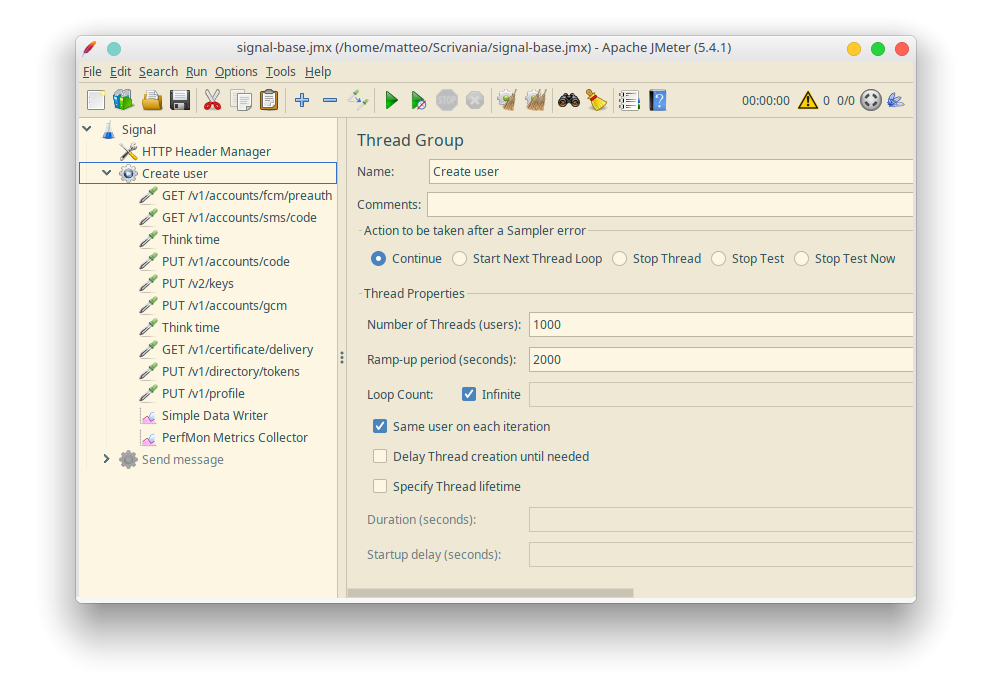
\includegraphics[width=\textwidth]{images/jmeter-steady-create}
    \caption{JMeter steady load for accounts creation}
    \label{fig:jmeterbaseuser}
\end{figure}

As the figure shows, the test performs one account creation for each user, with a number of threads at a time which gets incremented slowly. JMeter proceeds until it gets a manual interruption.

The same thing is done for the message sending steady load, as the following figure shows.

\begin{figure}[H]
    \centering
    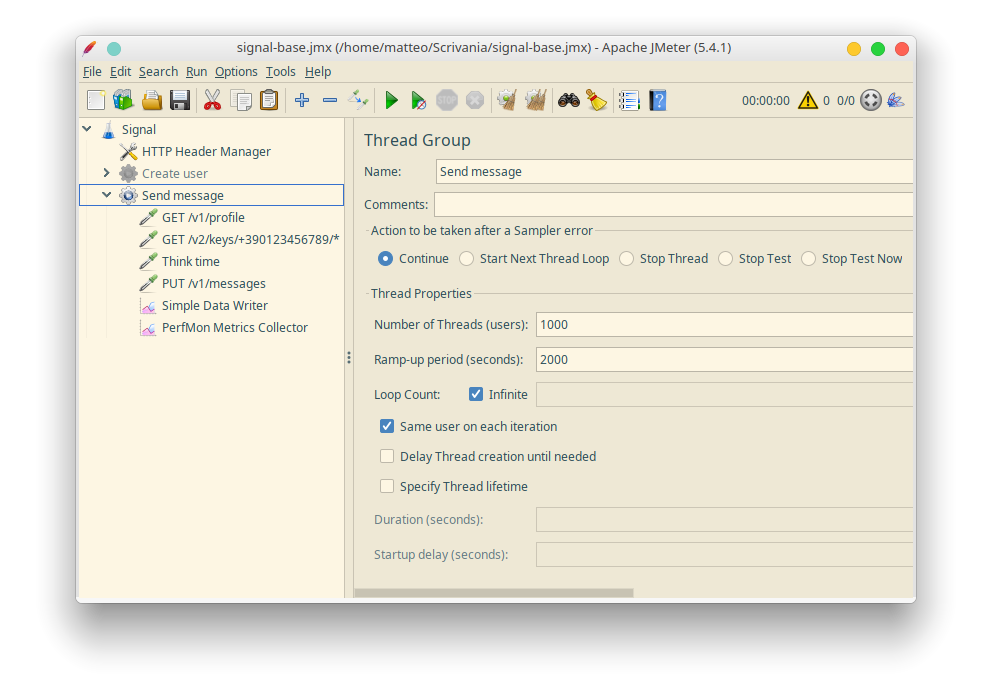
\includegraphics[width=\textwidth]{images/jmeter-steady-message}
    \caption{JMeter steady load for message sending}
    \label{fig:jmeterbasemessage}
\end{figure}

\subsection{Peak load settings\label{sec:highloadsettings}}

With peak load we mean a load much higher than the steady one, with a low duration, used to simulate a higher use of the Signal application. An example can be the New Year's Eve, where a lot of messages are sent in a specific period of time.

The load is high enough for the server because of the low capacity.
There is a limit of $200$ parallel users, who execute sequences of requests to the Signal APIs to create accounts or to send messages. Each user is added after $0.5$ seconds (ramp-up of $50$ seconds) and the experiment is repeated only once.

In order to perform a higher load test, for a shorter period of time, I used the following settings.
This time the maximum concurrent threads is set to $200$, with a ramp-up period of $50$ seconds (a thread is added every $0.5$ seconds), with $1$ cycle.

\begin{figure}[H]
    \centering
    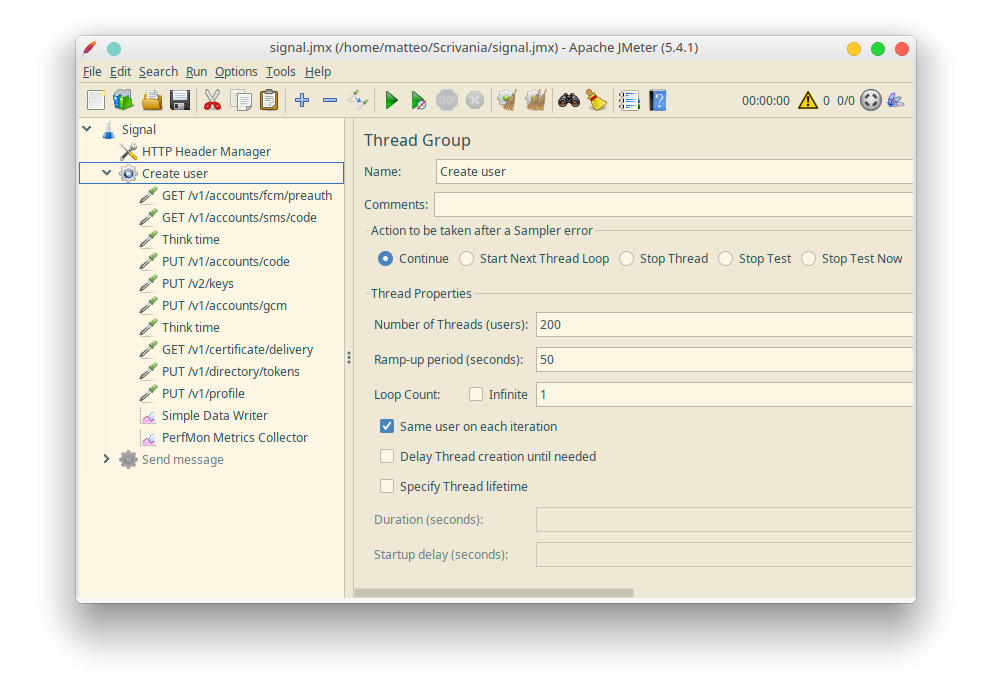
\includegraphics[width=\textwidth]{images/jmeter-peak-create}
    \caption{JMeter peak load for accounts creation}
    \label{fig:jmeterhighloadcreate}
\end{figure}

\clearpage

The same thing has been done for the message sending.

\begin{figure}[H]
    \centering
    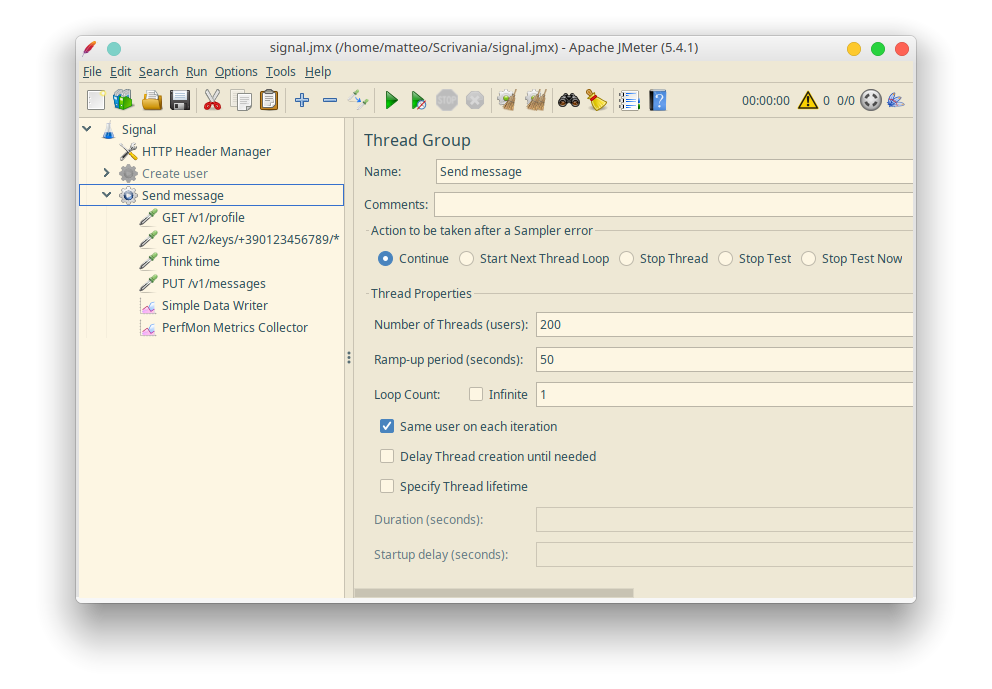
\includegraphics[width=\textwidth]{images/jmeter-peak-message}
    \caption{JMeter peak load for message sending}
    \label{fig:jmeterhighloadmessage}
\end{figure}

\subsection{Perfmon\label{sec:perfmon}}

Perfmon\footnote{\url{https://jmeter-plugins.org/wiki/PerfMon}} is a plugin made for JMeter which is used to collect metrics about the resources of the machine which is tested.
I used it to collect data about the CPU usage, the RAM usage and the network performance during the tests.

\begin{figure}[H]
    \centering
    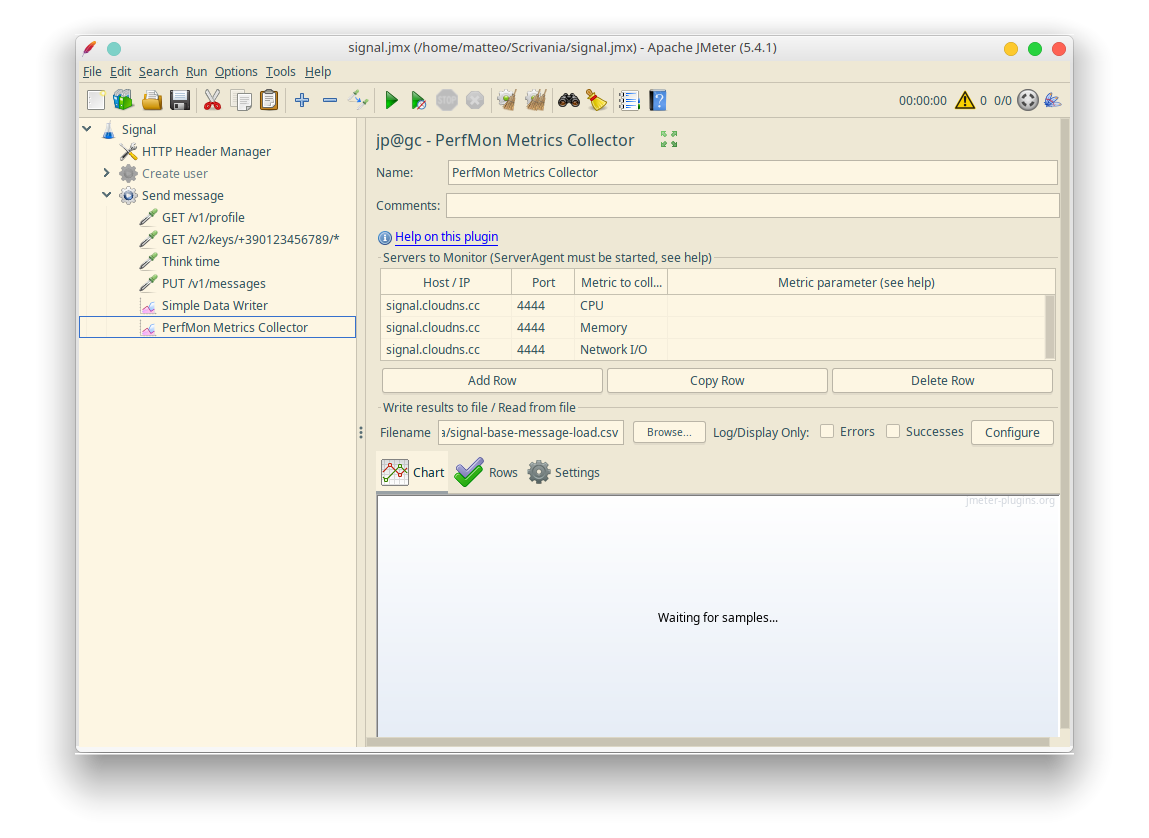
\includegraphics[width=\textwidth]{images/perfmon}
    \caption{JMeter Perfmon plugin}
    \label{fig:jmeterperfmon}
\end{figure}


\section{Results\label{sec:results}}

In this section I report the measures found by the test executions on both of the server versions, and some observations on them.

\subsection{New user registration\label{sec:newuser}}

All the Signal APIs are managed by the Dropwizard controllers, the framework used in order to implement the server orchestrator.

The experiment uses the following calls to the REST APIs of the Signal server:

\begin{table}[H]
\resizebox{\textwidth}{!}{%
\begin{tabular}{llll}
\hline
\multicolumn{1}{c}{\textbf{Type of request}} & \multicolumn{1}{c}{\textbf{Request path}} & \multicolumn{1}{c}{\textbf{Description}} & \multicolumn{1}{c}{\textbf{Involved components}} \\ \hline
GET & /v1/accounts/fcm/preauth & Request a preauth to Firebase Cloud Message & Dropwizard, Redis, PostgreSQL/DynamoDB, GCM \\
GET & /v1/accounts/sms/code & Request an OTP code, sent using Twilio & Dropwizard, Redis, PostgreSQL/DynamoDB, GCM, Twilio \\
PUT & /v1/accounts/code & Send the received code from Twilio & Dropwizard, Redis, PostgreSQL/DynamoDB, AWS SQS \\
PUT & /v2/keys & Send the keys for encryption protocol & Dropwizard, Redis, PostgreSQL/DynamoDB \\
PUT & /v1/accounts/gcm & Send details for Google Cloud Message & Dropwizard, Redis, PostgreSQL/DynamoDB, AWS SQS \\
GET & /v1/certificate/delivery & Get certificate from the Signal server & Dropwizard, Redis, PostgreSQL/DynamoDB \\
PUT & /v1/directory/tokens & Put tokens of Signal account & Dropwizard \\
PUT & /v1/profile & Put information of Signal account & Dropwizard,Redis, PostgreSQL/DynamoDB \\ \hline
\end{tabular}%
}
\caption{Sequence of calls to register a new account}
\label{tab:apiregistration}
\end{table}

\clearpage

Between the request for the Twilio OTP code and its insertion and between the insertion of the GCM data and the insertion of the profile data there are two intervals of $3$ seconds to simulate the user time to do an action with precompiled fields.

\subsubsection{Steady load on Signal 4.97}

From this experiment I expect to find some results which confirm that Signal 4.97 is easier to overload compared to the 6.13 version.
This is because the 4.97 version was the one used in production at the time of the outage.
So the response times should be high, and the experiment duration should be shorter than the one in 6.13 version.

Here there is a table with the measures obtained from the accounts' creation on Signal 4.97.

\begin{table}[H]
\resizebox{\textwidth}{!}{%
\begin{tabular}{@{}lllllllllll@{}}
\toprule
\multicolumn{1}{c}{\multirow{2}{*}{\textbf{Request}}} & \multicolumn{1}{c}{\multirow{2}{*}{\textbf{\#Samples}}} & \multicolumn{7}{c}{\textbf{Response times (ms)}} & \multicolumn{2}{c}{\textbf{Network (KB/s)}} \\ \cmidrule(l){3-11} 
\multicolumn{1}{c}{} & \multicolumn{1}{c}{} & \multicolumn{1}{c}{Average} & \multicolumn{1}{c}{Min} & \multicolumn{1}{c}{Max} & \multicolumn{1}{c}{Median} & \multicolumn{1}{c}{90th pct} & \multicolumn{1}{c}{95th pct} & \multicolumn{1}{c}{99th pct} & \multicolumn{1}{c}{Received} & \multicolumn{1}{c}{Sent} \\ \midrule
GET /v1/accounts/fcm/preauth & 3916 & 1709.69 & 17 & 96872 & 654.50 & 1959.50 & 3051.05 & 38072.90 & 3.70 & 3.19 \\
GET /v1/accounts/sms/code & 3858 & 1415.33 & 17 & 95211 & 664.00 & 2029.10 & 2308.10 & 5377.15 & 7.48 & 2.15 \\
GET /v1/certificate/delivery & 3677 & 1631.82 & 16 & 93170 & 845.00 & 2197.00 & 2787.20 & 6742.70 & 6.16 & 1.99 \\
PUT /v1/accounts/code & 3834 & 2923.34 & 17 & 94035 & 750.00 & 2059.00 & 3053.75 & 90726.65 & 4.17 & 3.93 \\
PUT /v1/accounts/gcm & 3683 & 1139.68 & 17 & 94560 & 784.00 & 2246.60 & 2693.80 & 4371.12 & 3.04 & 3.37 \\
PUT /v1/directory/tokens & 3652 & 1082.61 & 38 & 95104 & 802.50 & 2159.40 & 2514.75 & 4523.02 & 3.21 & 21.19 \\
PUT /v1/profile & 3648 & 949.07 & 21 & 94376 & 732.50 & 1942.10 & 2263.55 & 4689.34 & 3.09 & 4.31 \\
PUT /v2/keys & 3747 & 2537.98 & 47 & 95779 & 785.00 & 2203.80 & 2839.00 & 92842.44 & 3.34 & 28.59 \\ \bottomrule
\end{tabular}%
}
\caption{Steady load accounts' creation on Signal 4.97}
\label{tab:steadyloadcreation497}
\end{table}

From these data we can see that the calls used to save the keys request a higher time compared to the other requests.
This delay is due to the higher weight of the message, which contains a lot of keys, so it is heavier compared to the other messages.

All the requests which require read/write operations on a database involve Redis, which can trigger requests to PostgreSQL.
This is useful, Redis act as a database in RAM, so it is more efficient compared to PostgreSQL.

\begin{figure}[H]
    \centering
    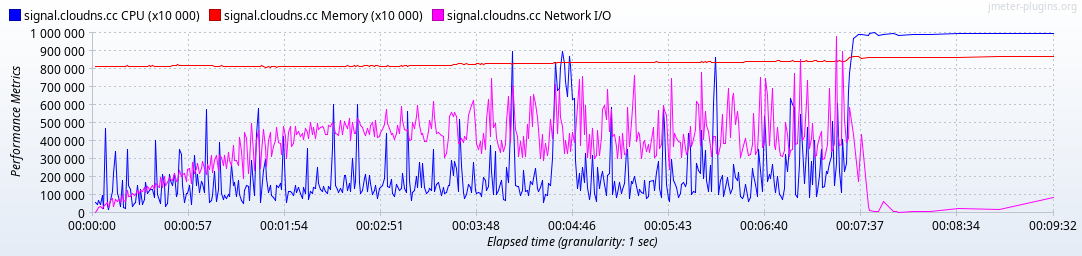
\includegraphics[width=\textwidth]{images/497/4.97-steady-create}
    \caption{Steady load accounts' creation on Signal 4.97}
    \label{fig:signalbasecreateloadold}
\end{figure}

From the diagram it is visible that the steady load increases gradually over time, with the traffic load. At $7:30$ the server reaches a breakpoint, the traffic goes to $0$ and the usage of CPU is stable at $100\%$.

\subsubsection{Peak load on Signal 4.97}

Comparing the situation to the previous experiment, here I do not expect to find an outage on the server. This time the results should highlight how the server reacts to the peak of load, and it is expected that they are worse compared to the 6.13 version.

Here I show the data obtained from the peak load for the accounts' creation.

\begin{table}[H]
\resizebox{\textwidth}{!}{%
\begin{tabular}{@{}lllllllllll@{}}
\toprule
\multicolumn{1}{c}{\multirow{2}{*}{\textbf{Request}}} & \multicolumn{1}{c}{\multirow{2}{*}{\textbf{\#Samples}}} & \multicolumn{7}{c}{\textbf{Response times (ms)}} & \multicolumn{2}{c}{\textbf{Network (KB/s)}} \\ \cmidrule(l){3-11} 
\multicolumn{1}{c}{} & \multicolumn{1}{c}{} & \multicolumn{1}{c}{Average} & \multicolumn{1}{c}{Min} & \multicolumn{1}{c}{Max} & \multicolumn{1}{c}{Median} & \multicolumn{1}{c}{90th pct} & \multicolumn{1}{c}{95th pct} & \multicolumn{1}{c}{99th pct} & \multicolumn{1}{c}{Received} & \multicolumn{1}{c}{Sent} \\ \midrule
GET /v1/accounts/fcm/preauth & 200 & 86.13 & 65 & 424 & 80.50 & 97.90 & 114.90 & 254.35 & 1.91 & 1.80 \\
GET /v1/accounts/sms/code & 200 & 23.87 & 18 & 90 & 22.00 & 26.90 & 40.00 & 65.89 & 4.17 & 1.22 \\
GET /v1/certificate/delivery & 200 & 23.17 & 17 & 146 & 21.00 & 25.00 & 36.95 & 68.94 & 3.57 & 1.18 \\
PUT /v1/accounts/code & 200 & 23.87 & 19 & 165 & 22.00 & 24.00 & 41.75 & 72.96 & 2.17 & 2.28 \\
PUT /v1/accounts/gcm & 200 & 21.96 & 18 & 75 & 21.00 & 24.00 & 28.90 & 51.98 & 1.78 & 1.99 \\
PUT /v1/directory/tokens & 200 & 44.56 & 38 & 161 & 42.00 & 47.00 & 62.85 & 99.91 & 1.89 & 12.55 \\
PUT /v1/profile & 200 & 29.61 & 23 & 99 & 27.00 & 33.00 & 49.00 & 79.78 & 1.83 & 2.56 \\
PUT /v2/keys & 200 & 59.21 & 47 & 113 & 57.00 & 69.90 & 73.95 & 110.88 & 1.78 & 16.85 \\ \bottomrule
\end{tabular}%
}
\caption{Peak load accounts' creation on Signal 4.97}
\label{tab:peakloadcreation497}
\end{table}

The table shows that the response times are lower compared to the ones obtained with the steady load. This is because a breakpoint is not reached, and all the requests receive a response from the server.

The requests with a higher response times are the preauth ones.

\begin{figure}[H]
    \centering
    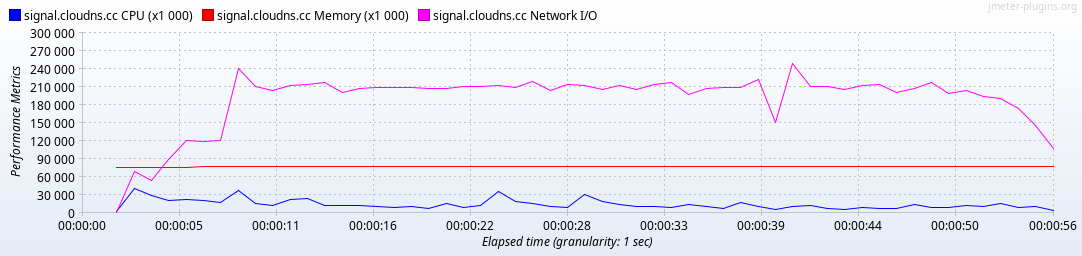
\includegraphics[width=\textwidth]{images/497/4.97-peak-create}
    \caption{Peak load accounts' creation on Signal 4.97}
    \label{fig:signalcreateloadold}
\end{figure}

The diagram shows that there is no overloading on the server, and all the requests receive a response.

Now I compare the obtained results with the 6.13 server version.

\subsubsection{Steady load on Signal 6.13}

In this experiment I expect that the results are worse, compared to the previous version.
The experiment, as for the version 4.97, is designed to create a steady load which slowly increments over time.

Here I report the results for the accounts' creation on Signal 6.13.

\begin{table}[H]
\resizebox{\textwidth}{!}{%
\begin{tabular}{@{}lllllllllll@{}}
\toprule
\multicolumn{1}{c}{\multirow{2}{*}{\textbf{Request}}} & \multicolumn{1}{c}{\multirow{2}{*}{\textbf{\#Samples}}} & \multicolumn{7}{c}{\textbf{Response times (ms)}} & \multicolumn{2}{c}{\textbf{Network (KB/s)}} \\ \cmidrule(l){3-11} 
\multicolumn{1}{c}{} & \multicolumn{1}{c}{} & \multicolumn{1}{c}{Average} & \multicolumn{1}{c}{Min} & \multicolumn{1}{c}{Max} & \multicolumn{1}{c}{Median} & \multicolumn{1}{c}{90th pct} & \multicolumn{1}{c}{95th pct} & \multicolumn{1}{c}{99th pct} & \multicolumn{1}{c}{Received} & \multicolumn{1}{c}{Sent} \\ \midrule
GET /v1/accounts/fcm/preauth & 1323 & 234.66 & 23 & 15185 & 97.00 & 382.60 & 487.60 & 1528.00 & 3.21 & 2.89 \\
GET /v1/accounts/sms/code & 1312 & 175.04 & 19 & 13576 & 74.50 & 315.70 & 405.35 & 586.09 & 6.25 & 1.95 \\
GET /v1/certificate/delivery & 1268 & 448.49 & 18 & 14760 & 80.50 & 356.00 & 480.95 & 13488.77 & 5.96 & 1.83 \\
PUT /v1/accounts/code & 1307 & 334.37 & 18 & 14909 & 85.00 & 346.20 & 448.20 & 12462.56 & 3.72 & 3.63 \\
PUT /v1/accounts/gcm & 1277 & 227.33 & 17 & 15074 & 73.00 & 323.00 & 405.50 & 930.90 & 2.92 & 3.13 \\
PUT /v1/directory/tokens & 1238 & 233.04 & 38 & 15143 & 100.00 & 358.20 & 421.05 & 1065.75 & 2.99 & 19.47 \\
PUT /v1/profile & 1233 & 249.62 & 20 & 14900 & 74.00 & 332.00 & 413.60 & 4343.24 & 3.97 & 3.93 \\
PUT /v2/keys & 1287 & 270.94 & 48 & 14315 & 110.00 & 349.00 & 457.60 & 1275.20 & 2.96 & 26.71 \\ \bottomrule
\end{tabular}%
}
\caption{Steady load on Signal 6.13}
\label{tab:steadyloadcreation613}
\end{table}

As the table shows, the response times are much lower than the 4.97 version of the server on average and on median times. This is due to the experiment duration, but also from the more efficient architecture, which uses AWS components.
Apart from this, the breakpoint is reached in a shorter time, so the architecture use components which have better performance but are more influenced by load.

\begin{figure}[H]
    \centering
    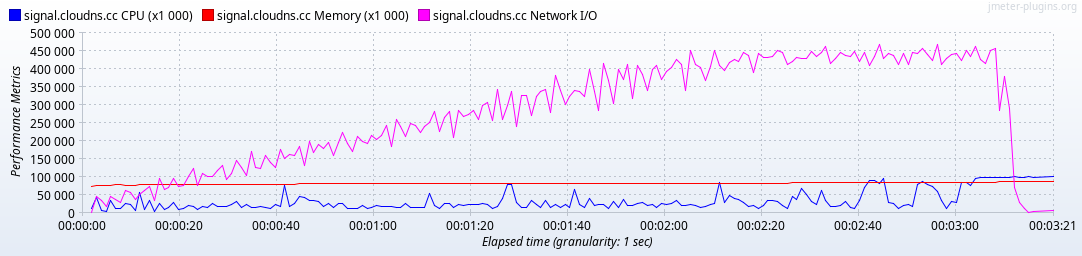
\includegraphics[width=\textwidth]{images/613/6.13-steady-create}
    \caption{Steady load accounts' creation on Signal 6.13}
    \label{fig:signalbasecreateloadnew}
\end{figure}

The diagram shows that the breakpoint is reached in about $3$ minutes from the start of the experiment, much less than the previous version.

The next section shows the peak load experiment.

\subsubsection{Peak load on Signal 6.13}

The results should show the behavior of the new Signal server to high load. I expect that the behavior is better compared to the previous version, as it uses DynamoDB and more AWS services.

Here there are the data related to the peak load experiment for the account creation.

\begin{table}[H]
\resizebox{\textwidth}{!}{%
\begin{tabular}{@{}lllllllllll@{}}
\toprule
\multicolumn{1}{c}{\multirow{2}{*}{\textbf{Request}}} & \multicolumn{1}{c}{\multirow{2}{*}{\textbf{\#Samples}}} & \multicolumn{7}{c}{\textbf{Response times (ms)}} & \multicolumn{2}{c}{\textbf{Network (KB/s)}} \\ \cmidrule(l){3-11} 
\multicolumn{1}{c}{} & \multicolumn{1}{c}{} & \multicolumn{1}{c}{Average} & \multicolumn{1}{c}{Min} & \multicolumn{1}{c}{Max} & \multicolumn{1}{c}{Median} & \multicolumn{1}{c}{90th pct} & \multicolumn{1}{c}{95th pct} & \multicolumn{1}{c}{99th pct} & \multicolumn{1}{c}{Received} & \multicolumn{1}{c}{Sent} \\ \midrule
GET /v1/accounts/fcm/preauth & 200 & 101.37 & 71 & 365 & 94.00 & 128.90 & 157.95 & 252.39 & 1.91 & 1.80 \\
GET /v1/accounts/sms/code & 200 & 29.96 & 22 & 90 & 26.00 & 39.00 & 57.90 & 77.99 & 3.89 & 1.23 \\
GET /v1/certificate/delivery & 200 & 26.18 & 17 & 114 & 22.00 & 38.90 & 57.75 & 109.88 & 3.59 & 1.18 \\
PUT /v1/accounts/code & 200 & 23.81 & 19 & 65 & 22.00 & 28.90 & 40.95 & 54.98 & 2.18 & 2.29 \\
PUT /v1/accounts/gcm & 200 & 23.24 & 17 & 81 & 22.00 & 27.90 & 39.90 & 50.00 & 1.79 & 2.00 \\
PUT /v1/directory/tokens & 200 & 44.37 & 39 & 88 & 42.00 & 48.00 & 62.85 & 80.95 & 1.90 & 12.62 \\
PUT /v1/profile & 200 & 34.56 & 20 & 169 & 31.00 & 44.90 & 58.00 & 130.52 & 2.49 & 2.57 \\
PUT /v2/keys & 200 & 60.59 & 48 & 110 & 58.00 & 72.00 & 75.95 & 105.95 & 1.79 & 16.94 \\ \bottomrule
\end{tabular}%
}
\caption{Peak load accounts' creation on Signal 6.13}
\label{tab:peakloadcreation613}
\end{table}

The response times on the table are comparable between the two server versions, so they are both able to handle the peak loads.

\begin{figure}[H]
    \centering
    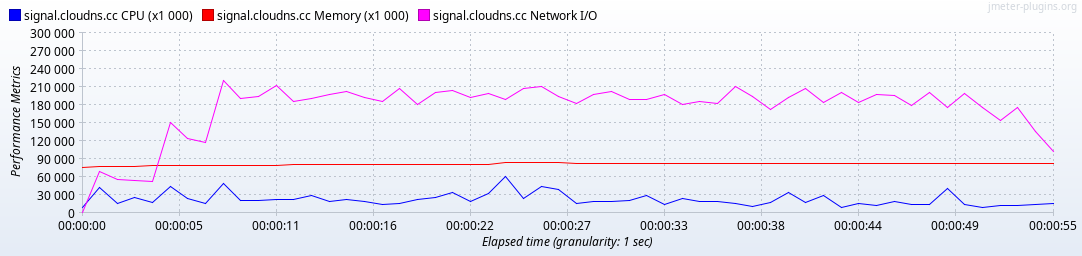
\includegraphics[width=\textwidth]{images/613/6.13-peak-create}
    \caption{Peak load accounts' creation on Signal 6.13}
    \label{fig:signalcreateloadnew}
\end{figure}

As on the 4.97 version, with the 6.13 version there are not overloads.
We can see that the percentage of CPU is lower on the 6.13 version of the server, which uses more AWS services instead of other services which require an internal management.

\subsection{New message sending\label{sec:newmessage}}

This experiment uses the following REST APIs:

\begin{table}[H]
\resizebox{\textwidth}{!}{%
\begin{tabular}{@{}llll@{}}
\hline
\multicolumn{1}{c}{\textbf{Type of request}} & \multicolumn{1}{c}{\textbf{Request path}} & \multicolumn{1}{c}{\textbf{Description}} & \multicolumn{1}{c}{\textbf{Involved components}} \\ \hline
GET & /v1/profile & Request data of the receiver profile & Dropwizard, Redis, PostgreSQL/DynamoDB \\
GET & /v2/keys/+390123456789/* & Get the keys for message encryption & Dropwizard, Redis, PostgreSQL/DynamoDB \\
PUT & /v1/messages & Send the message to the receiver & Dropwizard, Redis, PostgreSQL/DynamoDB \\\bottomrule
\end{tabular}%
}
\caption{Sequence of calls to send a message}
\label{tab:apimessage}
\end{table}

Between the request of the keys to send the message to the receiver and the request to send the message there is a think time of $3$ seconds, to simulate a low think time of the user when he writes the message.

\clearpage

\subsubsection{Steady load on Signal 4.97}

Results of this experiment should show that sending a message requires less resources than creating an account (for number of requests and involved components of the architecture).
Moreover, the results should be worse compared to the 6.13 version of the server.

Here I report the table with the results from the experiment on Signal 4.97.

\begin{table}[H]
\resizebox{\textwidth}{!}{%
\begin{tabular}{@{}lllllllllll@{}}
\toprule
\multicolumn{1}{c}{\multirow{2}{*}{\textbf{Request}}} & \multicolumn{1}{c}{\multirow{2}{*}{\textbf{\#Samples}}} & \multicolumn{7}{c}{\textbf{Response times (ms)}} & \multicolumn{2}{c}{\textbf{Network (KB/s)}} \\ \cmidrule(l){3-11} 
\multicolumn{1}{c}{} & \multicolumn{1}{c}{} & \multicolumn{1}{c}{Average} & \multicolumn{1}{c}{Min} & \multicolumn{1}{c}{Max} & \multicolumn{1}{c}{Median} & \multicolumn{1}{c}{90th pct} & \multicolumn{1}{c}{95th pct} & \multicolumn{1}{c}{99th pct} & \multicolumn{1}{c}{Received} & \multicolumn{1}{c}{Sent} \\ \midrule
GET /v1/profile & 48665 & 2083.32 & 23 & 130681 & 3032.00 & 3785.00 & 9200.95 & 35696.04 & 63.51 & 36.36 \\
GET /v2/keys/+391234567890/* & 48442 & 1920.06 & 17 & 129352 & 2989.00 & 3691.00 & 6656.70 & 10982.99 & 37.58 & 9.93 \\
PUT /v1/messages & 48300 & 2227.99 & 20 & 130654 & 3063.50 & 6985.40 & 9446.95 & 38666.65 & 19.67 & 31.07
\end{tabular}%
}
\caption{Steady load message sending on Signal 4.97}
\label{tab:steadyloadmessage497}
\end{table}

The results are not as expected, because the response times are higher compared to the accounts' creations. This is because the requests are heavier.

Here I show the diagram with the resource use.

\begin{figure}[H]
    \centering
    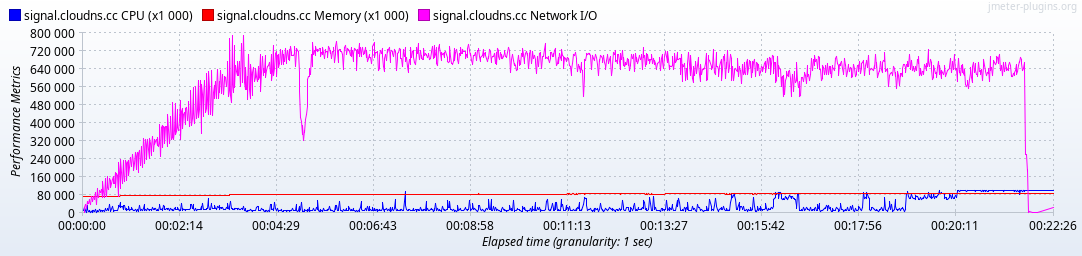
\includegraphics[width=\textwidth]{images/497/4.97-steady-message}
    \caption{Steady load message sending on Signal 4.97}
    \label{fig:signalbasemessageloadold}
\end{figure}

The diagram shows that the generated traffic is much higher compared to the previous experiment. Apart from this, the 4.97 version of the server needs at least $22$ minutes to reach an outage due to overload.

\subsubsection{Peak load on Signal 4.97}

As before, I expect that in this experiment the peak should be lower than the account creation for the same server version, while the response time should be higher than the 6.13 version.

Here there are the data relative to the experiment with peak load for sending messages.

\begin{table}[H]
\resizebox{\textwidth}{!}{%
\begin{tabular}{@{}lllllllllll@{}}
\toprule
\multicolumn{1}{c}{\multirow{2}{*}{\textbf{Request}}} & \multicolumn{1}{c}{\multirow{2}{*}{\textbf{\#Samples}}} & \multicolumn{7}{c}{\textbf{Response times (ms)}} & \multicolumn{2}{c}{\textbf{Network (KB/s)}} \\ \cmidrule(l){3-11} 
\multicolumn{1}{c}{} & \multicolumn{1}{c}{} & \multicolumn{1}{c}{Average} & \multicolumn{1}{c}{Min} & \multicolumn{1}{c}{Max} & \multicolumn{1}{c}{Median} & \multicolumn{1}{c}{90th pct} & \multicolumn{1}{c}{95th pct} & \multicolumn{1}{c}{99th pct} & \multicolumn{1}{c}{Received} & \multicolumn{1}{c}{Sent} \\ \midrule
GET /v1/profile & 200 & 96.74 & 78 & 508 & 89.00 & 109.90 & 123.90 & 397.77 & 6.07 & 4.05 \\
GET /v2/keys/+391234567890/* & 200 & 25.54 & 19 & 91 & 23.00 & 29.00 & 43.85 & 90.91 & 4.19 & 1.12 \\
PUT /v1/messages & 200 & 26.80 & 22 & 61 & 26.00 & 29.00 & 34.00 & 57.00 & 2.16 & 3.52
\end{tabular}%
}
\caption{Peak load message sending on Signal 4.97}
\label{tab:peakloadmessage497}
\end{table}

In this case the response times are comparable to the ones for the peak load of the accounts' creations.
The server is not overloaded, and each request gets a response.

\begin{figure}[H]
    \centering
    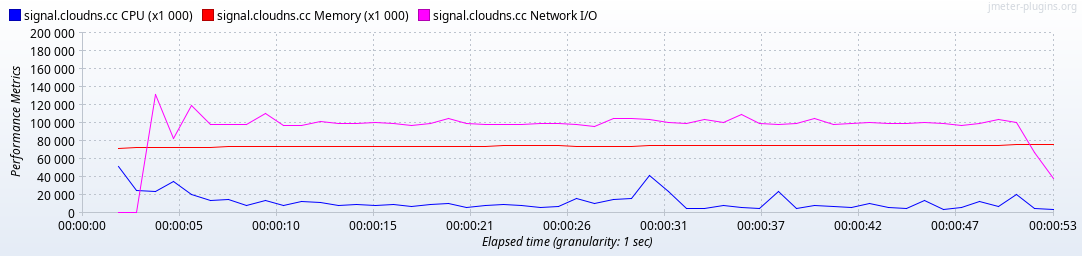
\includegraphics[width=\textwidth]{images/497/4.97-peak-message}
    \caption{Peak load message sending on Signal 4.97}
    \label{fig:signalmessageloadold}
\end{figure}

As the diagram shows, the CPU usage is comparable to the one for the accounts' creations, and the generated network traffic is lower.

Here I compare the previous results with the 6.13 Signal server version.

\subsubsection{Steady load on Signal 6.13}

Here the results should demonstrate that the 6.13 version of the server is able to handle a steady load for a higher duration compared to the 4.97 version, because the new server version involves more architectural components which use less resources on the server itself.
The results should be worse compared to the ones related to the accounts' creation on the same version of the server.

The following table has got the measures for the message sending on Signal 6.13.

\begin{table}[H]
\resizebox{\textwidth}{!}{%
\begin{tabular}{@{}lllllllllll@{}}
\toprule
\multicolumn{1}{c}{\multirow{2}{*}{\textbf{Request}}} & \multicolumn{1}{c}{\multirow{2}{*}{\textbf{\#Samples}}} & \multicolumn{7}{c}{\textbf{Response times (ms)}} & \multicolumn{2}{c}{\textbf{Network (KB/s)}} \\ \cmidrule(l){3-11} 
\multicolumn{1}{c}{} & \multicolumn{1}{c}{} & \multicolumn{1}{c}{Average} & \multicolumn{1}{c}{Min} & \multicolumn{1}{c}{Max} & \multicolumn{1}{c}{Median} & \multicolumn{1}{c}{90th pct} & \multicolumn{1}{c}{95th pct} & \multicolumn{1}{c}{99th pct} & \multicolumn{1}{c}{Received} & \multicolumn{1}{c}{Sent} \\ \midrule
GET /v1/profile & 352 & 57919.86 & 42 & 253103 & 609.00 & 217865.70 & 248695.65 & 252657.40 & 2.48 & 0.68 \\
GET /v2/keys/+391234567890/* & 209 & 11001.51 & 25 & 251773 & 52.00 & 462.00 & 30623.00 & 250584.10 & 0.72 & 0.18 \\
PUT /v1/messages & 199 & 1730.33 & 31 & 246506 & 55.00 & 2537.00 & 3366.00 & 6867.00 & 0.36 & 0.57
\end{tabular}%
}
\caption{Steady load message sending on Signal 6.13}
\label{tab:steadyloadmessage613}
\end{table}

The response times in this experiment are very high because it has been manually interrupted after much time from the overload of the server, so the last requests have a very high response time. We can compare the median time for the requests with the 4.97 version of the server, to see that the server itself is more efficient compared to the old version, but it gets overloaded in much less time.

\clearpage

The following diagram shows the resource usage.

\begin{figure}[H]
    \centering
    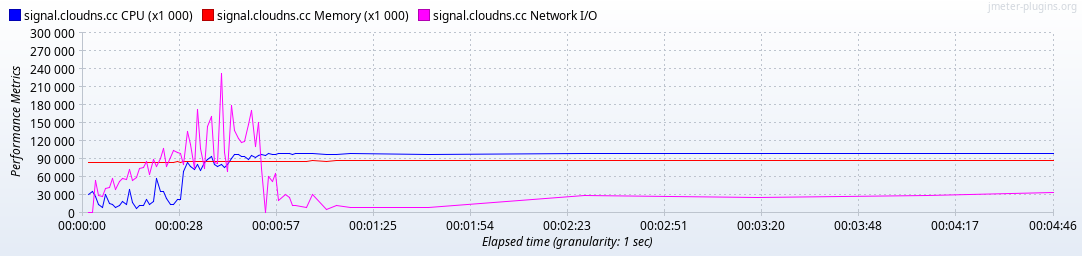
\includegraphics[width=\textwidth]{images/613/6.13-steady-message}
    \caption{Steady load message sending on Signal 6.13}
    \label{fig:signalbasemessageloadnew}
\end{figure}

The diagram clearly shows that the overload of the server happened at $30$ seconds from the start of the experiment. Much less network traffic has been generated.

On the next section there are the peak load results.

\subsubsection{Peak load on Signal 6.13}

Here I expect that the results show that the new version of the server requires less resources to manage a peak of traffic.
At the same time the response times should be lower compared to the ones for the peak load related to the accounts' creation.

Here the data relative to the peak load.

\begin{table}[H]
\resizebox{\textwidth}{!}{%
\begin{tabular}{@{}lllllllllll@{}}
\toprule
\multicolumn{1}{c}{\multirow{2}{*}{\textbf{Request}}} & \multicolumn{1}{c}{\multirow{2}{*}{\textbf{\#Samples}}} & \multicolumn{7}{c}{\textbf{Response times (ms)}} & \multicolumn{2}{c}{\textbf{Network (KB/s)}} \\ \cmidrule(l){3-11} 
\multicolumn{1}{c}{} & \multicolumn{1}{c}{} & \multicolumn{1}{c}{Average} & \multicolumn{1}{c}{Min} & \multicolumn{1}{c}{Max} & \multicolumn{1}{c}{Median} & \multicolumn{1}{c}{90th pct} & \multicolumn{1}{c}{95th pct} & \multicolumn{1}{c}{99th pct} & \multicolumn{1}{c}{Received} & \multicolumn{1}{c}{Sent} \\ \midrule
GET /v1/profile & 200 & 86.27 & 73 & 199 & 83.00 & 98.00 & 111.95 & 174.78 & 6.37 & 4.04 \\
GET /v2/keys/+391234567890/* & 200 & 22.94 & 18 & 53 & 22.00 & 25.00 & 29.00 & 46.97 & 3.96 & 1.11 \\
PUT /v1/messages & 200 & 25.68 & 21 & 56 & 24.00 & 30.00 & 42.00 & 54.97 & 2.14 & 3.48
\end{tabular}%
}
\caption{Peak load message sending on Signal 6.13}
\label{tab:peakloadmessage613}
\end{table}

We can see that the obtained results are comparable for average and median times with the 4.97 version of the server.
No overload takes place.

The next diagram shows the used resources.

\begin{figure}[H]
    \centering
    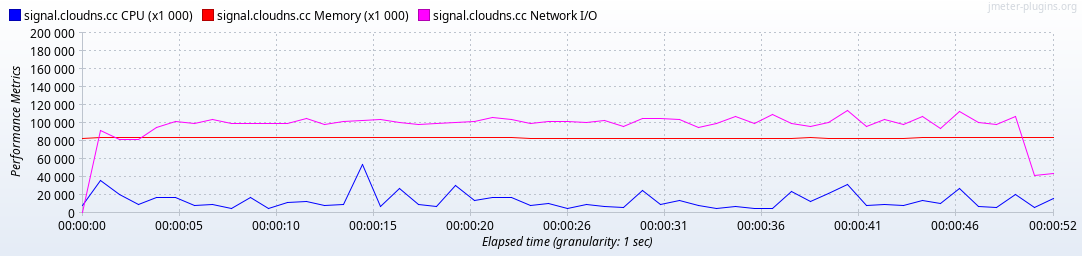
\includegraphics[width=\textwidth]{images/613/6.13-peak-message}
    \caption{Peak load message sending on Signal 6.13}
    \label{fig:signalhighmessageloadnew}
\end{figure}

In this case both the CPU usage and the network traffic are quite similar, there are no significant difference between the two server behaviors.